%
% teil3.tex -- Beispiel-File für Teil 3
%
% (c) 2020 Prof Dr Andreas Müller, Hochschule Rapperswil
%
% !TEX root = ../../buch.tex
% !TEX encoding = UTF-8
%
\section{Kombination von Möbius Transformationen
\label{moebius:section:teil3}}
\kopfrechts{Teil 3}


Möbius-Transformationen können als Kombination einfacher Transformationen wie Translation, Skalierung und Inversion dargestellt werden.

\textbf{Beispiel:}
\[
f(z) = \frac{2z + 3}{z + 1}
\]

Wir schreiben \( z \) in der Form:
\[
z = x + i
\]

Einsetzen ergibt:
\[
f(z) = \frac{2(x + i) + 3}{(x + i) + 1}
\]

Wobei wir zum rechnen z nehmen anstatt x+1

Nun formen wir den Zähler um:
\[
f(z) = \frac{2(z + 1) + 1}{z + 1}
\]

Aufteilen des Bruchs:
\[
f(z) = \frac{2(z + 1)}{z + 1} + \frac{1}{z + 1}
\]

Kürzen ergibt:
\[
f(z) = 2 + \frac{1}{z + 1}
\]

\textbf{Interpretation:}

Die Möbius-Transformation wird schrittweise zerlegt:

\[
z_1 = z + 1
\]
Dabei erfolgt eine Verschiebung der komplexen Ebene um \(1\) nach rechts.

\[
z_2 = \frac{1}{z_1}
\]
Hier wird eine Inversion durchgeführt. Punkte nahe beim Ursprung werden nach außen abgebildet und umgekehrt.

\[
f(z) = 2 + z_2
\]
Abschließend erfolgt eine weitere Verschiebung um \(2\) nach rechts.

Somit ergibt sich insgesamt die Transformation
\[
f(z) = \frac{2z + 3}{z + 1}.
\]

\begin{figure}[h]
	\centering
	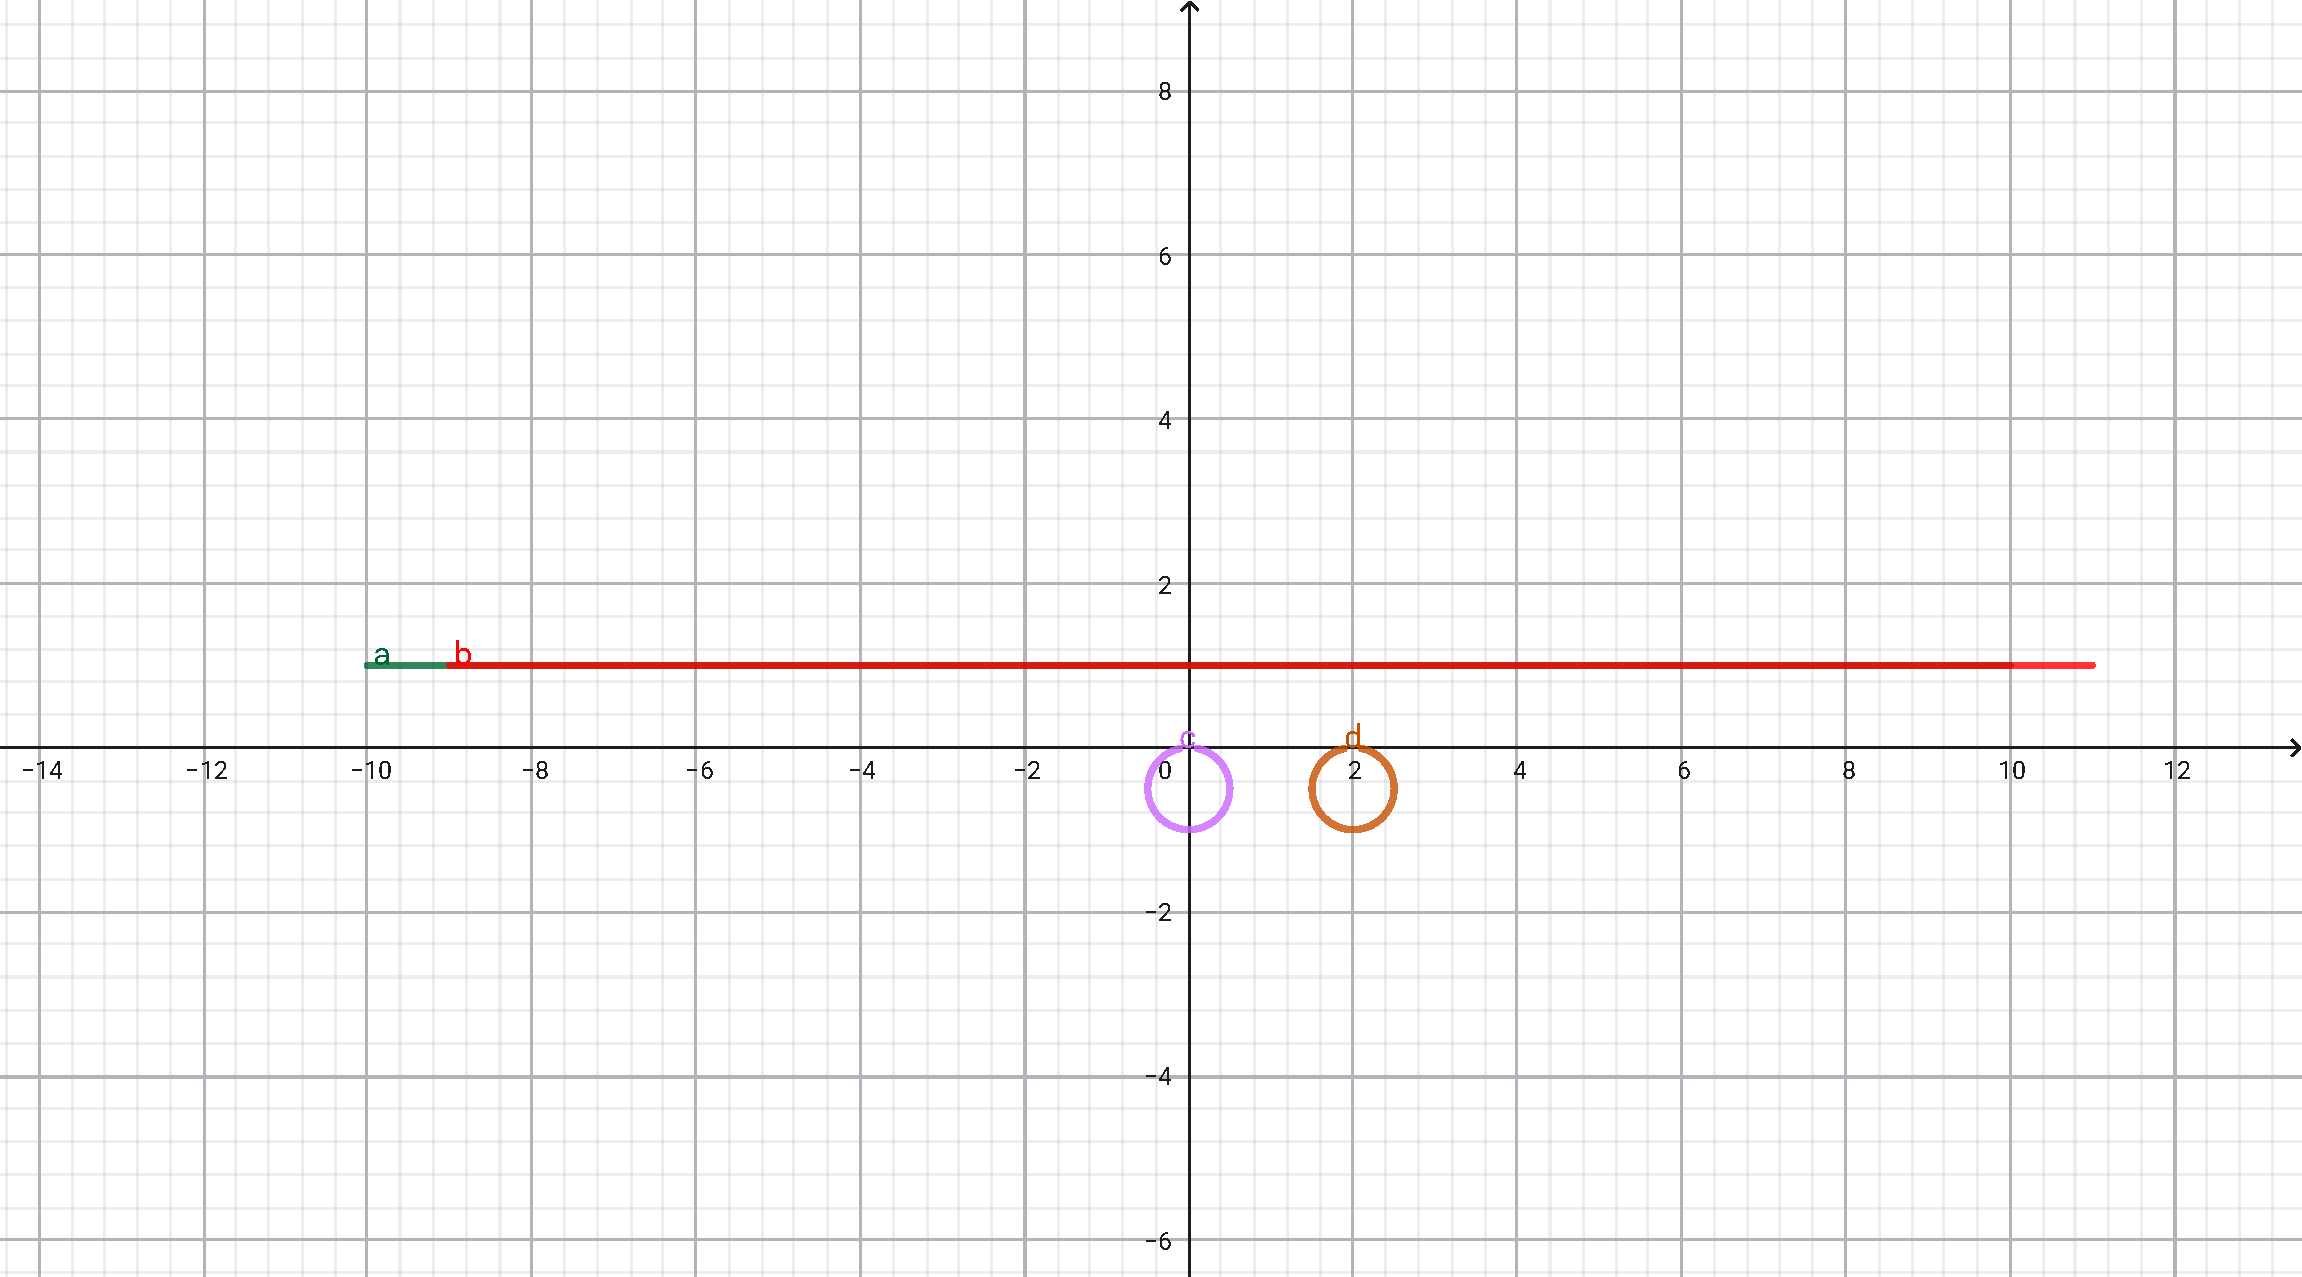
\includegraphics[width=0.6\textwidth]{bild6.pdf}
	\caption{Kombination der Translationen}
\end{figure} 

Auf der Abbildung 24.6 sieht man gut wie a unsere Startgerade ist, bei b die verschiebung um 1, bei c die Inversion von der Gerade zum Kreis, weil die Gerade nicht durch den Nullpunkt geht und bei d nochmals eine verschiebung um 2 stattfindet.
